\section{选择电动机}

\subsection{计算电动机所需功率}
输出功率
\begin{equation}
    P= \frac{T\omega}{9550}=\frac{2500 \times \frac{450}{2} \times 10^{-3} \times 80}{9550} = 9.42kw
\end{equation}

查表的各个传动装置的传动效率及其传动比

\begin{tabular}{|c|c|p{12em}|c|c|}
    \hline
    联轴器 & 球滚子轴承 & 斜齿圆柱齿轮(闭式传动,精度等级8级) & 圆柱齿轮(开式传动) & 运输滚筒 \\
    \hline
    0.99   & 0.99       & 0.97                                  & 0.96                 & 0.96     \\
    \hline
    1      & 1          & 3$\sim$6                              & 4$\sim$6             & 1        \\
    \hline
\end{tabular}

总传动效率为
\begin{equation}
    \eta = 0.99^4 \times 0.97 \times 0.96^2 = 0.859
\end{equation}

电动机所需额定功率

\begin{equation}
    P_d = \frac{P}{0.857} = 10.97
\end{equation}

\subsection{选择电动机}
查表得理论传动比范围是 12$\sim$36。可选择的电动机转速范围为:$n_d = i_a \times n = (12 \sim 36)\times 80=(960 \sim 2880)r/min$。总的电动机选择方案共有以下三种情况。

\begin{tabular}{|c|c|c|c|}
    \hline
    方案 & 电机型号      & 额定功率$kW$ & 同步转速$(r/min)$ \\
    \hline
    1    & $YE3-160M1-2$ & 11           & 2940              \\
    \hline
    2    & $YE3-160M-4$  & 11           & 1470              \\
    \hline
    3    & $YE3-160L-6$  & 11           & 975               \\
    \hline
\end{tabular}

考虑到低转速的电动机,转矩大,且传动装置的总传动比较小、体积小、重量较小。选定电动机型号为:$YE3-160L-6$,额定功率为$11kW$,同步转速为$975r/min$,重量为$140kg$.

\begin{figure}[h]
    \centering
    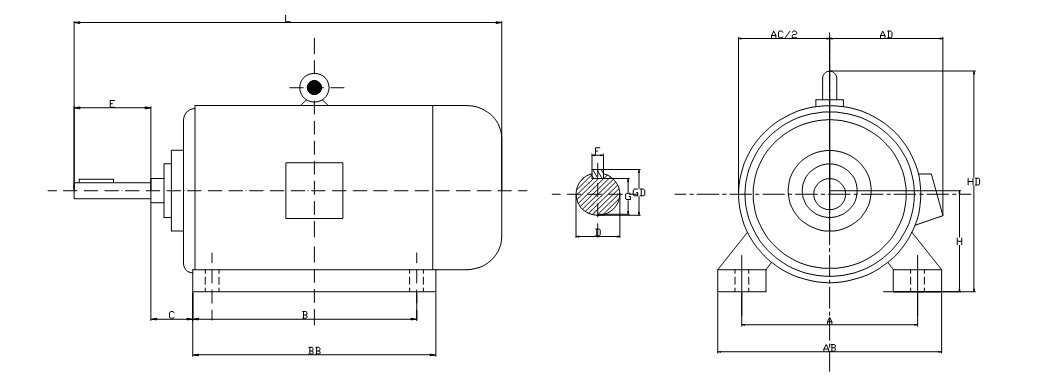
\includegraphics[scale=0.5]{graphic/3-1.png}
    \caption{电动机尺寸}
\end{figure}

\begin{tabular}{|c|p{8em}|c|c|c|c|}
    \hline
    中心高 & 外形尺寸                        & 底脚安装尺寸    & 地脚螺栓孔直径 & 轴伸尺寸        & 装键部位尺寸    \\
    \hline
    $H$    & $L\times (AC/2+AD)\times HD$    & $A\times B$     & $K$            & $D\times E$     & $F\times GD$    \\
    \hline
    160    & $760\times 380\times 425      $ & $254\times 253$ & $14.5      $   & $42\times 110 $ & $12\times 37  $ \\
    \hline
\end{tabular}

\subsection{分配各级传动比}
(1)总传动比的计算

由选定的电动机满载转速$n_m$和工作机主动轴的转速$n$,可得传动装置总传动比为
\begin{equation}
    i_a = \frac{n_m}{n} = \frac{975}{90} = 12.19
\end{equation}

(2)分配传动装置传动比

取高速级传动比为$i_a = 4.8 $, 则开式齿轮传动传动比为
\begin{equation}
    i_2 = \frac{i_a}{i_1}=2.5
\end{equation}

\subsection{计算各轴转速、功率和转矩}
\subsubsection{电动机输出参数}
\[
    P_0 = 10.97kW
\]
\[
    n_0 = n =975r/min
\]
\[
    T_0 = 9550\times \frac{P_0}{n_0}= \frac{10.97}{975} = 107.45N \cdot m
\]

\subsubsection{高速轴的参数}
\[
    P_1 = P_0 \times \eta_1 = 10.97 \times 1 =10.97 kW
\]
\[
    n_1 = n_0 =975 r/min
\]
\[
    T_1 = T_0 \times i_0 \times \eta_{01} = 107.45 N \cdot m
\]

\subsubsection{低速轴的参数}
\[
    P_2 = P_1 \times \eta_{2} \eta_{3} = 10.53 kW
\]
\[
    n_2 = \frac{n}{n_1} = 203.13 r/min
\]
\[
    T_2 = T_1 \times \eta_{2} \eta_{3} = 495.13 N \cdot m
\]
\subsubsection{工作机轴的参数}
\[
    P_3 = P_2 \times \eta_{2} \eta_{3} = 10.11 kW
\]
\[
    n_3 = \frac{n_2}{i_2} = 81.25r/min
\]
\[
    T_3 = T_2 \times \eta_{2} \eta_{3} = 1188.31N \cdot m \\
\]

各轴运动和动力参数的计算结果汇总于下表

\begin{tabular}{|c|c|c|c|c|}
    \hline
    轴名称              & 电机轴   & 高速轴   & 低速轴   & 工作机轴  \\
    \hline
    转速$n/(r/min)$     & $975$    & $ 975$   & $203.13$ & 81.25     \\
    \hline
    功率$P/kW$          & $10.97$  & $10.97$  & $10.53$  & $10.11$ \\
    \hline
    转矩$T/(N \cdot m)$ & $107.45$ & $107.45$ & $495.13$  & $1188.31$   \\
    \hline
\end{tabular}